Resumen de las principales características de las variables relevantes en los registros de logs de navegación. Análisis de la distribución de los datos, incluyendo medidas de centralidad y dispersión. Usando la librería Pandas de Python, podemos obtener información importante sobre los conjuntos de datos. Estos valores nos proporcionarán un mayor entendimiento de la composición y estructura de los registros de navegación.

Podemos obtener información respecto a la cantidad de valores faltantes en el dataframe que se está utilizando, los cuales suman 36,853 en total. De estos datos faltantes, 36,853 corresponden principalmente al campo 'canal', con solo un valor faltante en el campo 'método'. Como se vio en el capítulo anterior, estos valores fueron eliminados del dataframe.

Haciendo uso de la misma librería, podemos determinar los tipos de datos que contiene cada campo:

\begin{itemize}
    \item \textbf{rut:} Contiene datos de tipo string.
    \item \textbf{fecha:} Contiene datos de tipo date.
    \item \textbf{metodo:} Contiene datos de tipo string.
    \item \textbf{canal:} Contiene datos de tipo string.
\end{itemize}

Además se puede conocer la cantidad de valores únicos que posee cada una de las columnas del dataframe (luego del proceso ETL):

\begin{itemize}
    \item \textbf{rut cliente:} Contiene 35,524 valores únicos.
    \item \textbf{fecha:} Contiene 21,148 valores únicos.
    \item \textbf{metodo:} Contiene 85 valores únicos.
    \item \textbf{canal:} Contiene 2 valores únicos.
\end{itemize}

Ahora veremos la frecuencia con la que aparecen los valores más frecuentes en cada campo:
\begin{itemize}
    \item Para rut el valor más común es 'MTU0NjM5NzIx' y tiene una frecuencia de 320,689.
    \item Para método el valor más común es 'getAccountWithdrawal()' y tiene una frecuencia de 259,733.
    \item Para el canal el más común es 'PWA' con una frecuencia de 1,029,538.
    \item Para el campo fecha es distinto ya que cada registro posee valores distintos, esto se debe al detalle del valor guardado ya que este llega a considerar las milesimas de segundos.
\end{itemize}

Ahora veremos un gráfico que representa la distribución de los métodos en el conjunto de datos. En esta ocasión, se presentarán únicamente los diez métodos que tienen la mayor frecuencia, dado que la cantidad de métodos registrados es demasiado grande para ser mostrada en un solo gráfico.

\begin{figure}[H]
    \begin{minipage}[t]{0.9\textwidth}
        \caption{Distribución de métodos en el dataset.}
        \label{frecuencia-metodos}        
    \end{minipage}

    \vspace{10pt}

    \begin{minipage}[b]{1.0\textwidth}
        \centering
        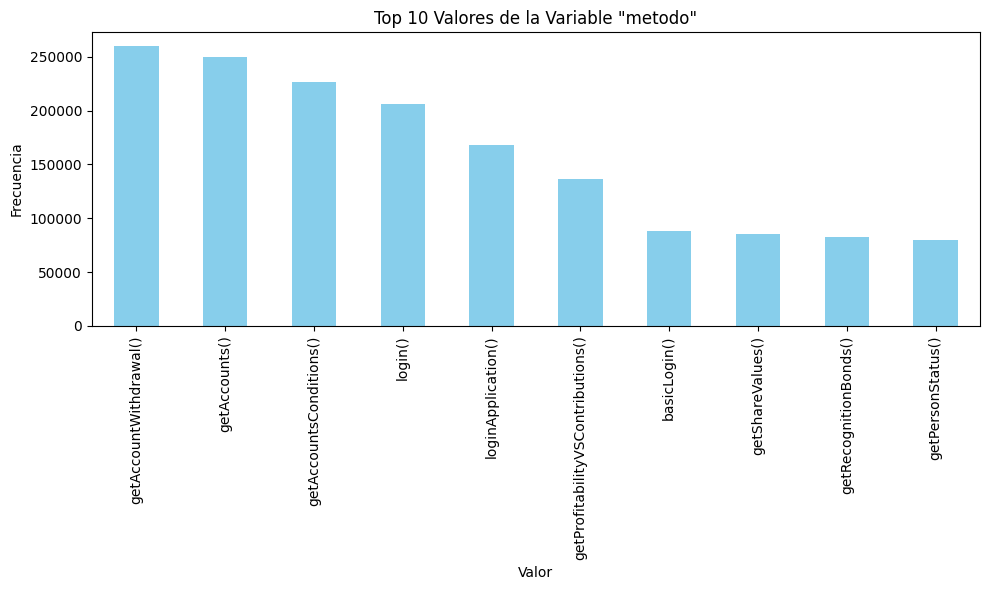
\includegraphics[width=\textwidth]{img/frecuencia-metodo.png}        
    \end{minipage}

    \begin{minipage}[t]{0.9\textwidth}
        Fuente: Elaboración propia.
    \end{minipage}
\end{figure}

\sloppy
La distribución muestra que las actividades relacionadas con cuentas (getAccountWithdrawal(), getAccounts(), y getAccountsConditions()) son las más frecuentes. Esto sugiere que la mayoría de los usuarios están interesados en la gestión y consulta de sus cuentas. Por otro lado, las actividades como login() y loginApplication() también tienen una alta frecuencia, indicando que el proceso de inicio de sesión es común, lo cual es esperado en una plataforma segura. De acá podemos podemos concluir que las actividades más populares pueden ser un área clave para la mejora continua y la optimización de la experiencia del usuario. Las actividades menos frecuentes no deben ser ignoradas; se debe evaluar su importancia y cómo pueden ser promocionadas o mejoradas.

Para analizar las fechas, se decidió realizar una descripción de estas por día y hora. Año y mes quedan fuera del análisis ya que todos los datos pertenecen al mismo año y mes. Respecto a los días, en el set de datos hay un total de ocho días, y están presentes las veinticuatro horas del día. Estas tienen una frecuencia de:

\subsubsection{Distribución de días:}
\begin{itemize}
    \item Se cuenta con un rango de 8 días consecutivos, comenzando en el día 14 y finalizando en el día 20. Cada día está asociado con un número que refleja una cantidad particular, con el día 14 teniendo la mayor cantidad de 4689, y el día 20 la menor con 138.
    % \item 14: 4689
    % \item 13: 4598
    % \item 15: 4026
    % \item 16: 2991
    % \item 17: 2619
    % \item 18: 1877
    % \item 19: 211
    % \item 20: 138
\end{itemize}

\subsubsection{Distribución de horas:}
\begin{itemize}
    \item Se observa una distribución de métricas a lo largo de las 24 horas del día. Las horas con las mayores cantidades se presentan al inicio de la tarde, con la hora 14 liderando con 1382 unidades. La actividad disminuye progresivamente hacia las horas nocturnas, siendo la hora 22 la última con una cantidad significativa de 1055 unidades antes de una reducción notable durante las horas de madrugada. Las horas menos activas son las primeras horas de la mañana, con la hora 5 registrando la menor cantidad de 438 unidades.
    % \item 14: 1382
    % \item 15: 1263
    % \item 13: 1240
    % \item 16: 1123
    % \item 22: 1055
    % \item 19: 1042
    % \item 18: 1037
    % \item 21: 1022
    % \item 3: 1009
    % \item 12: 999
    % \item 23: 992
    % \item 20: 985
    % \item 17: 921
    % \item 00: 890
    % \item 1: 859
    % \item 2: 800
    % \item 4: 787
    % \item 11: 726
    % \item 10: 605
    % \item 9: 540
    % \item 8: 514
    % \item 6: 463
    % \item 7: 457
    % \item 5: 438
\end{itemize}

Al analizar la distribución de los días, se observa que los días 14 y 13 presentan la mayor frecuencia en los registros, con 4689 y 4598 eventos, respectivamente. A medida que avanzan los días, se nota una disminución significativa en la cantidad de registros, llegando a solo 138 eventos el día 20.

En cuanto a la distribución de las horas, se puede observar que las horas 14, 15 y 13 tienen las frecuencias más altas, con 1382, 1263 y 1240 eventos, respectivamente. Las horas entre las 16 y las 21 también muestran una frecuencia considerablemente alta, mientras que las horas más tempranas (de 00 a 04) y las horas de la madrugada (después de las 04) presentan menor actividad, siendo la hora 05 la menos frecuente con 438 eventos.

Este análisis detallado por días y horas proporciona una visión más completa sobre la distribución temporal de los eventos registrados en el conjunto de datos, lo que puede ser útil para comprender los patrones de comportamiento de los usuarios en la plataforma.